% Options for packages loaded elsewhere
\PassOptionsToPackage{unicode}{hyperref}
\PassOptionsToPackage{hyphens}{url}
\PassOptionsToPackage{dvipsnames,svgnames,x11names}{xcolor}
\documentclass[
  10pt,
  fontset=fandol]{ctexart}
\usepackage{xcolor}
\usepackage[margin=16mm]{geometry}
\usepackage{amsmath,amssymb}
\setcounter{secnumdepth}{-\maxdimen} % remove section numbering
\usepackage{iftex}
\ifPDFTeX
  \usepackage[T1]{fontenc}
  \usepackage[utf8]{inputenc}
  \usepackage{textcomp} % provide euro and other symbols
\else % if luatex or xetex
  \usepackage{unicode-math} % this also loads fontspec
  \defaultfontfeatures{Scale=MatchLowercase}
  \defaultfontfeatures[\rmfamily]{Ligatures=TeX,Scale=1}
\fi
\usepackage{lmodern}
\ifPDFTeX\else
  % xetex/luatex font selection
\fi
% Use upquote if available, for straight quotes in verbatim environments
\IfFileExists{upquote.sty}{\usepackage{upquote}}{}
\IfFileExists{microtype.sty}{% use microtype if available
  \usepackage[]{microtype}
  \UseMicrotypeSet[protrusion]{basicmath} % disable protrusion for tt fonts
}{}
\makeatletter
\@ifundefined{KOMAClassName}{% if non-KOMA class
  \IfFileExists{parskip.sty}{%
    \usepackage{parskip}
  }{% else
    \setlength{\parindent}{0pt}
    \setlength{\parskip}{6pt plus 2pt minus 1pt}}
}{% if KOMA class
  \KOMAoptions{parskip=half}}
\makeatother
\usepackage{longtable,booktabs,array}
\newcounter{none} % for unnumbered tables
\usepackage{calc} % for calculating minipage widths
% Correct order of tables after \paragraph or \subparagraph
\usepackage{etoolbox}
\makeatletter
\patchcmd\longtable{\par}{\if@noskipsec\mbox{}\fi\par}{}{}
\makeatother
% Allow footnotes in longtable head/foot
\IfFileExists{footnotehyper.sty}{\usepackage{footnotehyper}}{\usepackage{footnote}}
\makesavenoteenv{longtable}
\usepackage{graphicx}
\makeatletter
\newsavebox\pandoc@box
\newcommand*\pandocbounded[1]{% scales image to fit in text height/width
  \sbox\pandoc@box{#1}%
  \Gscale@div\@tempa{\textheight}{\dimexpr\ht\pandoc@box+\dp\pandoc@box\relax}%
  \Gscale@div\@tempb{\linewidth}{\wd\pandoc@box}%
  \ifdim\@tempb\p@<\@tempa\p@\let\@tempa\@tempb\fi% select the smaller of both
  \ifdim\@tempa\p@<\p@\scalebox{\@tempa}{\usebox\pandoc@box}%
  \else\usebox{\pandoc@box}%
  \fi%
}
% Set default figure placement to htbp
\def\fps@figure{htbp}
\makeatother
\setlength{\emergencystretch}{3em} % prevent overfull lines
\providecommand{\tightlist}{%
  \setlength{\itemsep}{0pt}\setlength{\parskip}{0pt}}
\usepackage{amsmath,amssymb,mathtools,needspace}
\xeCJKDeclareCharClass{CJK}{"2032,"0400->"04FF,"2160->"216B,"2460->"2473,"25A0,"25C7,"25CB,"25CF}
\IfFontExistsTF{Arial Unicode MS}{\xeCJKsetup{AutoFallBack=true}\setCJKfallbackfamilyfont{\CJKrmdefault}{Arial Unicode MS}}{}
\setcounter{secnumdepth}{0}
\setlength{\emergencystretch}{2em}
\allowdisplaybreaks
\usepackage{bookmark}
\IfFileExists{xurl.sty}{\usepackage{xurl}}{} % add URL line breaks if available
\urlstyle{same}
\hypersetup{
  pdftitle={正交多项式},
  colorlinks=true,
  linkcolor={Maroon},
  filecolor={Maroon},
  citecolor={Blue},
  urlcolor={Blue},
  pdfcreator={LaTeX via pandoc}}

\title{正交多项式}
\author{}
\date{}

\begin{document}
\maketitle

\subsection{3.4 正交多项式}\label{ux6b63ux4ea4ux591aux9879ux5f0f}

\subsubsection{3.4.1 正交化手续}\label{ux6b63ux4ea4ux5316ux624bux7eed}

定义3.9 设 \(g_n(x)\) 是首项系数 \(a_n \neq 0\) 的 \(n\) 次多项式，如果多项式序列 \(g_0(x)\), \(g_1(x)\), \(\cdots\) 满足 \[
(g_j, g_k) = \int_a^b \rho(x) g_j(x) g_k(x) \mathrm{d}x = \begin{cases} 0, & j \neq k, \\ A_k > 0, & j = k \end{cases} \quad (j, k = 0, 1, \cdots),
\] 则称多项式序列 \(g_0(x), g_1(x), \cdots\) 在 \([a, b]\) 上带权 \(\rho(x)\) 正交，并称 \(g_n(x)\) 是 \([a, b]\) 上带权 \(\rho(x)\) 的 \(n\) 次正交多项式.

一般来说，当权函数 \(\rho(x)\) 及区间 \([a, b]\) 给定以后，可以由线性无关的一组基 \(\{1,\allowbreak  x,\allowbreak  x^2,\allowbreak  \cdots,\allowbreak  x^n,\allowbreak  \cdots\}\) 并利用正交化方法构造出正交多项式 \[
g_0(x) = 1, \quad g_n(x) = x^n - \sum_{k=0}^{n-1} \frac{(x^n, g_k)}{(g_k, g_k)} \cdot g_k(x), \quad k = 1, 2, \cdots.
\] 这样构造的正交多项式有以下性质： (1) \(g_n(x)\) 是最高项系数为 1 的 \(n\) 次多项式. (2) 任一 \(n\) 次多项式 \(P_n(x) \in H_n\) 均可表示为 \(g_0(x), g_1(x), \cdots, g_n(x)\) 的线性组合. (3) 当 \(n \neq m\) 时，\((g_n, g_m) = 0\) 且 \(g_n(x)\) 与任一次数小于 \(n\) 的多项式正交. (4) 有递推关系 \[
g_{n+1}(x) = (x - \alpha_n)g_n(x) - \beta_n g_{n-1}(x), \quad n = 0, 1, \cdots,
\] 其中 \[
g_0(x) = 1, \quad g_{n-1}(x) = 0,
\] \[
\alpha_n = \frac{(xg_n, g_n)}{(g_n, g_n)}, \quad n = 0, 1, \cdots,
\] \[
\beta_n = \frac{(g_n, g_n)}{(g_{n-1}, g_{n-1})}, \quad n = 1, 2, \cdots.
\] 这里 \((xg_n, g_n) = \int_a^b xg_n^2(x) \rho(x) \mathrm{d}x.\) (5) 设 \(g_0(x), g_1(x), \cdots\) 是在 \([a, b]\) 上带权 \(\rho(x)\) 的正交多项式序列，则 \(g_n(x)\) (\(n \geq 1\)) 的 \(n\) 个根都是单重实根，且都在区间 \((a, b)\) 内. 以上性质的证明可参看相关文献. 下面主要给出几类常见的而又十分重要的正交多项式.

\subsubsection{3.4.2 Legendre多项式}\label{legendreux591aux9879ux5f0f}

当区间为 \([-1, 1]\)、权函数 \(\rho(x) \equiv 1\) 时，由 \(\{1,\allowbreak  x,\allowbreak  x^2,\allowbreak  \cdots,\allowbreak  x^n,\allowbreak  \cdots\}\) 正交化得到的多

\begin{quote}
校注（agent 补充，原书索引疑误）：本页正交化构造式末尾原印``\(k=1,2,\cdots\)''，而 \(k\) 已是求和哑指标，外部序号应为 \(n=1,2,\cdots\)；转录保留原式。
\end{quote}

\begin{quote}
校注（agent 补充，原书初值疑误）：递推初值原印 \(g_{n-1}(x)=0\)，按原文保留。若对一般 \(n\) 成立，会与 \(g_0(x)=1\) 冲突；递推通常应以 \(g_{-1}(x)=0\) 开始。
\end{quote}

\href{../../source-images/pdf-071.jpeg}{查看原页}

项式就称为 Legendre 多项式, 并用 \(P_0(x), P_1(x), \cdots, P_n(x), \cdots\) 表示. 这是 Legendre 于 1785 年引进的. 1814 年 Rodrigul 给出了简单的表达式

\[
P_0(x) = 1, \quad P_n(x) = \frac{1}{2^n n!} \frac{\mathrm{d}^n}{\mathrm{d}x^n} \{(x^2 - 1)^n\} \quad (n = 1, 2, \cdots). \tag{3.4.1}
\]

由于 \((x^2 - 1)^n\) 是 \(2n\) 次多项式, 求 \(n\) 阶导数后得

\[
P_n(x) = \frac{1}{2^2 n!} (2n)(2n - 1) \cdots (n + 1)x^n + a_{n-1}x^{n-1} + \cdots + a_0,
\]

于是得首项 \(x^n\) 的系数 \(a_n = \frac{(2n)!}{2^n (n!)^2}\). 显然最高项系数为 1 的 Legendre 多项式为

\[
\tilde{P}_n(x) = \frac{n!}{(2n)!} \frac{\mathrm{d}^n}{\mathrm{d}x^n} [(x^2 - 1)^n]. \tag{3.4.2}
\]

Legendre 多项式有以下几个重要性质.

性质 1 正交性

\[
\int_{-1}^{1} P_n(x) P_m(x) \mathrm{d}x = \begin{cases} 0, & m \neq n, \\ \frac{2}{2n + 1}, & m = n. \end{cases} \tag{3.4.3}
\]

证明 令 \(\varphi(x) = (x^2 - 1)^n\), 则

\[
\varphi^{(k)}(\pm 1) = 0 \quad (k = 0, 1, \cdots, n - 1).
\]

设 \(Q(x)\) 是区间 \([-1, 1]\) 上 \(n\) 阶连续可微的函数, 由分部积分知

\[
\int_{-1}^{1} P_n(x) Q(x) \mathrm{d}x = \frac{1}{2^n n!} \int_{-1}^{1} Q(x) \varphi^{(n)}(x) \mathrm{d}x = -\frac{1}{2^n n!} \int_{-1}^{1} Q'(x) \varphi^{(n-1)}(x) \mathrm{d}x
\]

\[
= \cdots = \frac{(-1)^n}{2^n n!} \int_{-1}^{1} Q^{(n)}(x) \varphi(x) \mathrm{d}x.
\]

下面分两种情况讨论.

\begin{enumerate}
\def\labelenumi{(\arabic{enumi})}
\tightlist
\item
  若 \(Q(x)\) 是次数小于 \(n\) 的多项式, 则 \(Q^{(n)}(x) \equiv 0\), 故当 \(m \neq n\) 时, 有
\end{enumerate}

\[
\int_{-1}^{1} P_m(x) P_n(x) \mathrm{d}x = 0.
\]

\begin{enumerate}
\def\labelenumi{(\arabic{enumi})}
\setcounter{enumi}{1}
\tightlist
\item
  若
\end{enumerate}

\[
Q(x) = P_n(x) = \frac{1}{2^n n!} \varphi^{(n)}(x) = \frac{(2n)!}{2^n (n!)^2} x^n + \cdots,
\]

\[
Q^{(n)}(x) = P_n^{(n)}(x) = \frac{(2n)!}{2^n n!},
\]

则

\[
\int_{-1}^{1} P_n^2(x) \mathrm{d}x = \frac{(-1)^n (2n)!}{2^{2n} (n!)^2} \int_{-1}^{1} (x^2 - 1)^n \mathrm{d}x = \frac{(2n)!}{2^{2n} (n!)^2} \int_{-1}^{1} (1 - x^2)^n \mathrm{d}x.
\]

由于

\[
\int_{0}^{1} (1 - x^2)^n \mathrm{d}x = \int_{0}^{\frac{\pi}{2}} \cos^{2n+1} t \mathrm{d}t = \frac{2 \cdot 4 \cdots 2n}{1 \cdot 3 \cdots (2n+1)},
\]

故当 \(m = n\) 时, 有

\[
\int_{-1}^{1} P_n^2(x) \mathrm{d}x = \frac{2}{2n+1}.
\]

证毕.

\begin{quote}
校注（agent 补充，原书系数疑误）：由 \((x^2-1)^n\) 求导后写出的 \(P_n(x)\) 首项系数中，原分母明确印为 \(2^2n!\)，此处按原文保留。依据式 (3.4.1)，该处应为 \(2^nn!\)；这也与紧随其后的 \(a_n=(2n)!/[2^n(n!)^2]\) 一致。
\end{quote}

\href{../../source-images/pdf-072.jpeg}{查看原页}

性质 2 奇偶性 \[
P_n(-x) = (-1)^n P_n(x). \tag{3.4.4}
\]

由于 \(\varphi(x) = (x^2 - 1)^n\) 是偶次多项式，经过偶次求导仍为偶次多项式，经过奇次求导则为奇次多项式，故 \(n\) 为偶数时 \(P_n(x)\) 为偶函数，\(n\) 为奇数时 \(P_n(x)\) 为奇函数，于是式(3.4.4)成立.

性质 3 递推关系 考虑 \(n+1\) 次多项式 \(xP_n(x)\)，它可表示为 \[
xP_n(x) = a_0P_0(x) + a_1P_1(x) + \cdots + a_{n+1}P_{n+1}(x),
\] 两边乘以 \(P_k(x)\)，并从 \(-1\) 到 \(1\) 积分，得 \[
\int_{-1}^{1} xP_n(x)P_k(x) \mathrm{d}x = a_k \int_{-1}^{1} P_k^2(x) \mathrm{d}x.
\] 当 \(k \leqslant n-2\) 时，\(xP_k(x)\) 次数不大于 \(n-1\)，上式左端积分为零，故得 \(a_k = 0\). 当 \(k=n\) 时 \(xP_n^2(x)\) 为奇函数，左端积分仍为零，故 \(a_n = 0\). 于是 \[
xP_n(x) = a_{n-1}P_{n-1}(x) + a_{n+1}P_{n+1}(x),
\] 其中 \[
a_{n-1} = \frac{2n-1}{2} \int_{-1}^{1} xP_n(x)P_{n-1}(x) \mathrm{d}x = \frac{2n-1}{2} \frac{2n}{4n^2-1} = \frac{n}{2n+1},
\] \[
a_{n+1} = \frac{2n+3}{2} \int_{-1}^{1} xP_n(x)P_{n+1}(x) \mathrm{d}x = \frac{2n+3}{2} \frac{2(n+1)}{(2n+1)(2n+3)} = \frac{n+1}{2n+1},
\] 从而得到以下的递推公式： \[
(n+1)P_{n+1}(x) = (2n+1)xP_n(x) - nP_{n-1}(x) \quad (n=1,2,\cdots). \tag{3.4.5}
\] 由 \(P_0(x)=1\)，\(P_1(x)=x\)， 利用式(3.4.5)就可推出 \[
P_2(x) = (3x^2 - 1)/2,
\] \[
P_3(x) = (5x^3 - 3x)/2,
\] \[
P_4(x) = (35x^4 - 30x^2 + 3)/8,
\] \[
P_5(x) = (63x^5 - 70x^3 + 15x)/8,
\] \[
P_6(x) = (231x^6 - 315x^4 + 105x^2 - 5)/16,
\] \[
\vdots
\] 图 3.4给出了 \(P_0(x), P_1(x), P_2(x), P_3(x)\) 的图形.

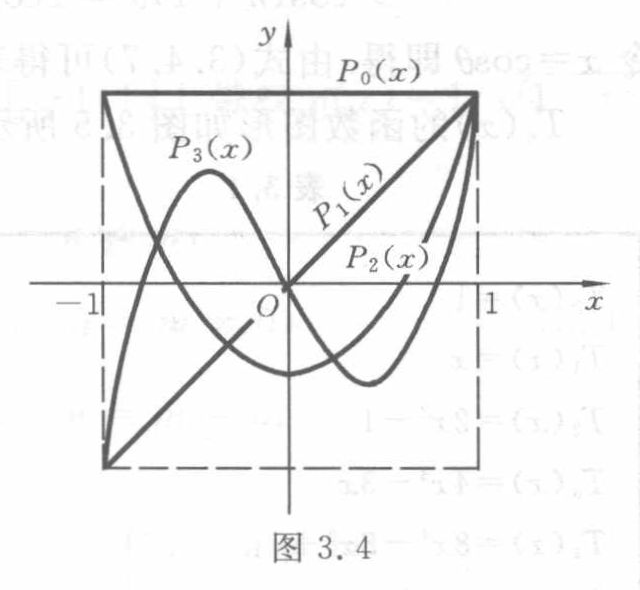
\includegraphics[width=0.85\linewidth,height=\textheight,keepaspectratio,alt={图 3.4 原图裁切}]{../assets/ch03a/fig-3-4.png}

图 3.4（原图）。Legendre 多项式 \(P_0(x)\)、\(P_1(x)\)、\(P_2(x)\)、\(P_3(x)\) 的图形。全部标签：\(x\)、\(y\)、\(O\)、\(-1\)、\(1\)、\(P_0(x)\)、\(P_1(x)\)、\(P_2(x)\)、\(P_3(x)\)；图中包含区间端点处的竖向及下边界虚线。

性质 4 在所有最高项系数为 1 的 \(n\) 次多项式中，Legendre 多项式 \(\widetilde{P}_n(x)\) 在 \([-1,1]\) 上与零的平方误差最小.

设 \(Q_n(x)\) 是任意一个最高项系数为 1 的 \(n\) 次多项式，它可表示为

\href{../../source-images/pdf-073.jpeg}{查看原页}

\[
Q_n(x) = \tilde{P}_n(x) + \sum_{k=0}^{n-1} a_k \tilde{P}_k(x) ,
\] 于是 \[
(Q_n, Q_n) = \int_{-1}^{1} Q_n^2(x) \mathrm{d}x = (\tilde{P}_n, \tilde{P}_n) + \sum_{k=0}^{n-1} a_k^2 (\tilde{P}_k, \tilde{P}_k) \geqslant (\tilde{P}_n, \tilde{P}_n)
\] 当且仅当 \(a_0 = a_1 = \cdots = a_{n-1} = 0\) 时等号才成立，即当 \(Q_n(x) \equiv \tilde{P}_n(x)\) 时平方误差最小.

性质 5 \(P_n(x)\) 在区间 \((-1, 1)\) 内有 \(n\) 个不同的实零点.

\subsubsection{3.4.3 Chebyshev多项式}\label{chebyshevux591aux9879ux5f0f}

当权函数 \(\rho(x) = \frac{1}{\sqrt{1-x^2}}\), 区间为 \([-1, 1]\) 时, 由序列 \(\{1,\allowbreak  x,\allowbreak  x^2,\allowbreak  \cdots,\allowbreak  x^n,\allowbreak  \cdots\}\) 正交化得到的正交多项式就是 Chebyshev多项式, 它可表示为 \[
T_n(x) = \cos(n \arccos x), \quad |x| \leqslant 1. \tag{3.4.6}
\] 若令 \(x = \cos \theta\), 则 \[
T_n(x) = \cos n \theta, \quad 0 \leqslant \theta \leqslant \pi.
\] Chebyshev多项式有很多重要性质.

性质 1 递推关系 \[
T_0(x) = 1, \quad T_1(x) = x,
\] \[
T_{n+1}(x) = 2xT_n(x) - T_{n-1}(x) \quad (n = 1, 2, \cdots). \tag{3.4.7}
\] 这只要由三角恒等式 \[
\cos(n+1)\theta = 2\cos \theta \cos n \theta - \cos(n-1)\theta \quad (n \geqslant 1)
\] 令 \(x = \cos \theta\) 即得. 由式(3.4.7)可得表 3.1.

\(T_n(x)\) 的函数图形如图 3.5 所示.

表 3.1

{\def\LTcaptype{none} % do not increment counter
\begin{longtable}[]{@{}ll@{}}
\toprule\noalign{}
多项式 & 表达式 \\
\midrule\noalign{}
\endhead
\bottomrule\noalign{}
\endlastfoot
\(T_0(x)\) & \(1\) \\
\(T_1(x)\) & \(x\) \\
\(T_2(x)\) & \(2x^2-1\) \\
\(T_3(x)\) & \(4x^3-3x\) \\
\(T_4(x)\) & \(8x^4-8x^2+1\) \\
\(T_5(x)\) & \(16x^5-20x^3+5x\) \\
\(T_6(x)\) & \(32x^6-48x^4+18x^2-1\) \\
\(T_7(x)\) & \(64x^7-112x^5+56x^3-7x\) \\
\(T_8(x)\) & \(128x^8-256x^6+160x^4-32x^2+1\) \\
\end{longtable}
}

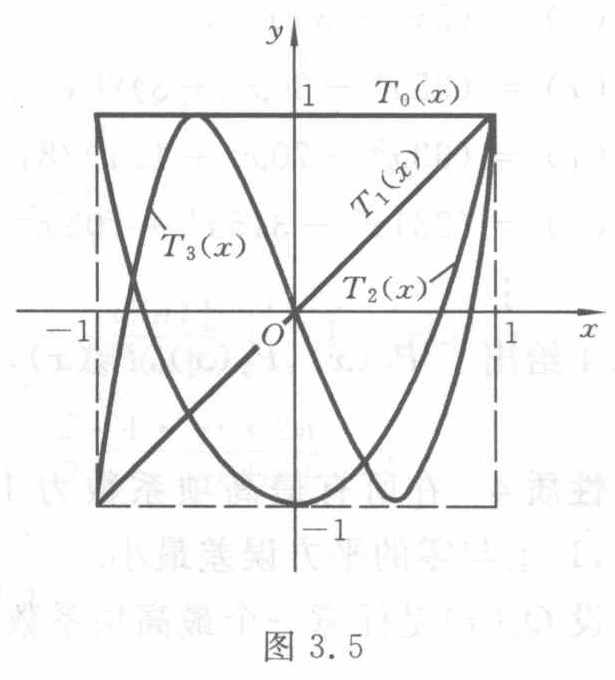
\includegraphics[width=0.85\linewidth,height=\textheight,keepaspectratio,alt={图 3.5 原图裁切}]{../assets/ch03a/fig-3-5.png}

图 3.5（原图）。Chebyshev 多项式 \(T_0(x)\)、\(T_1(x)\)、\(T_2(x)\)、\(T_3(x)\) 的图形。全部标签：\(x\)、\(y\)、\(O\)、横轴的 \(-1\)、\(1\)、纵轴的 \(1\)、\(-1\)、\(T_0(x)\)、\(T_1(x)\)、\(T_2(x)\)、\(T_3(x)\)；在 \(x=\pm1\) 处画有辅助线。

\href{../../source-images/pdf-074.jpeg}{查看原页}

由递推关系式(3.4.7)还可得到 \(T_n(x)\) 的最高项系数是 \(2^{n-1}(n \geqslant 1)\).

性质 2 \(T_n(x)\) 对零的偏差最小. 它可写成如下定理.

定理 3.7 在区间 \([-1,1]\) 上所有最高项系数为 1 的一切 \(n\) 次多项式中, \(\omega_n(x) = \frac{1}{2^{n-1}} T_n(x)\) 与零的偏差最小, 其偏差为 \(\frac{1}{2^{n-1}}\).

证明 由于 \(\omega_n(x) = \frac{1}{2^{n-1}} T_n(x) = x^n - P_{n-1}^*(x)\),

\[
\max_{-1 \leqslant x \leqslant 1} |\omega_n(x)| = \frac{1}{2^{n-1}} \max_{-1 \leqslant x \leqslant 1} |T_n(x)| = \frac{1}{2^{n-1}} ,
\] 且点 \(x_k = \cos \frac{k}{n}\pi (k=0,1,\cdots,n)\) 是 \(T_n(x)\) 的 Chebyshev 交错点组, 由定理 3.4 可知, 在区间 \([-1,1]\) 上, \(x^n\) 在 \(H_{n-1}\) 中最佳逼近多项式为 \(P_{n-1}^*(x)\), 即 \(\omega_n(x)\) 是与零的偏差最小的多项式. 证毕.

例 3.3 求 \(f(x) = 2x^3 + x^2 + 2x - 1\) 在 \([-1,1]\) 上的最佳二次逼近多项式.

解 由题意, 所求最佳逼近多项式 \(P_{2}^*(x)\) 应满足

\[
\max_{-1 \leqslant x \leqslant 1} |f(x) - P_{2}^*(x)| = \min .
\] 由定理 3.6 可知, 当

\[
f(x) - P_{2}^*(x) = \frac{1}{2} T_3(x) = 2x^3 - \frac{3}{2}x
\] 时, 与零偏差最小, 故

\[
P_{2}^*(x) = f(x) - \frac{1}{2} T_3(x) = x^2 + \frac{7}{2}x - 1
\] 就是 \(f(x)\) 在 \([-1,1]\) 上的最佳二次逼近多项式.

性质 3 Chebyshev 多项式 \(\{T_k(x)\}\) 在区间 \([-1,1]\) 上带权 \(\rho(x) = 1 / \sqrt{1-x^2}\) 正交, 且

\[
\int_{-1}^{1} \frac{T_n(x)T_m(x)\,\mathrm{d}x}{\sqrt{1-x^2}} = \begin{cases} 0, & n \neq m, \\ \frac{\pi}{2}, & n = m \neq 0, \\ \pi, & n = m = 0. \end{cases} \tag{3.4.8}
\]

事实上, 令 \(x = \cos \theta\), 则 \(\mathrm{d}x = -\sin \theta \mathrm{d}\theta\), 于是

\[
\int_{-1}^{1} \frac{T_n(x)T_m(x)}{\sqrt{1-x^2}} \mathrm{d}x = \int_{0}^{\pi} \cos n\theta \cos m\theta \mathrm{d}\theta = \begin{cases} 0, & n \neq m, \\ \frac{\pi}{2}, & n = m \neq 0, \\ \pi, & n = m = 0. \end{cases}
\]

性质 4 \(T_{2k}(x)\) 只含 \(x\) 的偶次幂, \(T_{2k+1}(x)\) 只含 \(x\) 的奇次幂.

此性质由递推关系直接得到.

\begin{quote}
校注（agent 补充，原书交叉引用疑误）：例 3.3 中原文写``由定理 3.6 可知''，照录。此处使用的是本页定理 3.7 的最小偏差性质；定理 3.6 是线性无关与内积行列式的判别条件。
\end{quote}

\href{../../source-images/pdf-075.jpeg}{查看原页}

性质 5 \(T_n(x)\) 在区间 \([-1,1]\) 上有 \(n\) 个零点 \(x_k = \cos \frac{2k-1}{2n}\pi, k=1, \cdots, n\). 此外, 实际计算中时常要求 \(x^n\) 用 \(T_0, T_1, \cdots, T_n\) 的线性组合表示, 其公式为 \[
x^n = 2^{1-n} \sum_{k=0}^{[\frac{n}{2}]} \binom{n}{k} T_{n-2k}(x). \tag{3.4.9}
\]

这里规定 \(T_0 = 1/2\). \(n=1 \sim 8\) 的结果如表 3.2 所示.

表 3.2

{\def\LTcaptype{none} % do not increment counter
\begin{longtable}[]{@{}ll@{}}
\toprule\noalign{}
幂函数 & Chebyshev 多项式表示 \\
\midrule\noalign{}
\endhead
\bottomrule\noalign{}
\endlastfoot
\(1\) & \(T_0\) \\
\(x\) & \(T_1\) \\
\(x^2\) & \(\frac12(T_0+T_2)\) \\
\(x^3\) & \(\frac14(3T_1+T_3)\) \\
\(x^4\) & \(\frac18(3T_0+4T_2+T_4)\) \\
\(x^5\) & \(\frac1{16}(10T_1+5T_3+T_5)\) \\
\(x^6\) & \(\frac1{32}(10T_0+15T_2+6T_4+T_6)\) \\
\(x^7\) & \(\frac1{64}(35T_1+21T_3+7T_5+T_7)\) \\
\(x^8\) & \(\frac1{128}(35T_0+56T_2+28T_4+8T_6+T_8)\) \\
\end{longtable}
}

\subsubsection{3.4.4 其他常用的正交多项式}\label{ux5176ux4ed6ux5e38ux7528ux7684ux6b63ux4ea4ux591aux9879ux5f0f}

一般地说, 如果区间 \([a,b]\) 及权函数 \(\rho(x)\) 不同, 则得到的正交多项式也不同. 除上述两种最重要的正交多项式外, 下面再给出三种较常用的正交多项式.

\paragraph{1. 第二类 Chebyshev 多项式}\label{ux7b2cux4e8cux7c7b-chebyshev-ux591aux9879ux5f0f}

在区间 \([-1,1]\) 上带权 \(\rho(x) = \sqrt{1-x^2}\) 的正交多项式称为第二类 Chebyshev 多项式, 其表达式为

\[
U_n(x) = \frac{\sin[(n+1)\arccos x]}{\sqrt{1-x^2}}. \tag{3.4.10}
\]

由 \(x=\cos\theta\) 可得

\[
\int_{-1}^{1} U_n(x) U_m(x) \sqrt{1-x^2} \mathrm{d}x = \int_{0}^{\pi} \sin(n+1)\theta \sin(m+1)\theta \mathrm{d}\theta
\]

\[
= \left\{ \begin{array}{l l} 0, & m \neq n, \\ \frac{\pi}{2}, & m=n, \end{array} \right.
\]

\begin{quote}
校注（agent 补充，记号约定）：式 (3.4.9) 后原文规定 \(T_0=1/2\)，而表 3.2 首行原印 \(1=T_0\)；两处均忠实保留。式 (3.4.9) 的求和使用临时的半权常数项约定，表 3.2 则与前文通常定义 \(T_0=1\) 一致。使用时须区分这两种约定。
\end{quote}

\href{../../source-images/pdf-076.jpeg}{查看原页}

即 \(\{U_n(x)\}\) 是区间 \([-1,1]\) 上带权 \(\rho(x)=\sqrt{1-x^2}\) 的正交多项式族。还可得到递推关系式

\[
U_0(x)=1,\quad U_1(x)=2x,
\]

\[
U_{n+1}(x)=2xU_n(x)-U_{n-1}(x)\quad(n=1,2,\cdots).
\]

\paragraph{2. Laguerre 多项式}\label{laguerre-ux591aux9879ux5f0f}

在区间 \([0,\infty)\) 上带权 \(\rho(x)=\mathrm e^{-x}\) 的正交多项式称为 Laguerre 多项式，其表达式为

\[
L_n(x)=\mathrm e^n\frac{\mathrm d^n}{\mathrm dx^n}(x^n\mathrm e^{-x}).\tag{3.4.11}
\]

它也具有正交性质

\[
\int_0^\infty \mathrm e^{-x}L_n(x)L_m(x)\,\mathrm dx=
\begin{cases}
0,&m\ne n,\\
(n!)^2,&m=n
\end{cases}
\]

和递推关系

\[
L_0(x)=1,\quad L_1(x)=1-x,
\]

\[
L_{n+1}(x)=(1+2n-x)L_n(x)-n^2L_{n-1}(x)\quad(n=1,2,\cdots).
\]

\paragraph{3. Hermite 多项式}\label{hermite-ux591aux9879ux5f0f}

在区间 \((-\infty,\infty)\) 上带权 \(\rho(x)=\mathrm e^{-x^2}\) 的正交多项式称为 Hermite 多项式，其表达式为

\[
H_n(x)=(-1)^n\mathrm e^{x^2}\frac{\mathrm d^n}{\mathrm dx^n}(\mathrm e^{-x^2}).\tag{3.4.12}
\]

它满足正交关系

\[
\int_{-\infty}^{+\infty}\mathrm e^{-x^2}H_m(x)H_n(x)\,\mathrm dx=
\begin{cases}
0,&m\ne n,\\
2^nn!\sqrt\pi,&m=n,
\end{cases}
\]

并有递推关系

\[
H_0(x)=1,\quad H_1(x)=2x,
\]

\[
H_{n+1}(x)=2xH_n(x)-2nH_{n-1}(x)\quad(n=1,2,\cdots).
\]

\begin{center}\rule{0.5\linewidth}{0.5pt}\end{center}

\subsection{相关原页校注（agent 补充）}\label{ux76f8ux5173ux539fux9875ux6821ux6ce8agent-ux8865ux5145}

以下校注来自本节覆盖的原页，可能也涉及同页相邻小节；原文照录与校正说明分开保留。

\subsubsection{原书 PDF 页 76 的校注}\label{ux539fux4e66-pdf-ux9875-76-ux7684ux6821ux6ce8}

\href{../pages/pdf-076.md}{完整原页转录} · \href{../../source-images/pdf-076.jpeg}{原页图像}

校注记录：ch03b-E001。

\begin{quote}
校注（agent 补充）：式 (3.4.11) 的原扫描明确印为 \(\mathrm e^n\)，已忠实保留；这是疑似原书错误，不是 OCR 误读。取 \(n=0\)，原式给出 \(L_0(x)=\mathrm e^{-x}\)，与紧接着印出的 \(L_0(x)=1\) 矛盾。相容的 Rodrigues 表达式前因子应为 \(\mathrm e^x\)。见 \href{../assets/ch03b/p076-laguerre-formula.png}{原式放大裁切}。
\end{quote}

\subsection{本节覆盖原页的校注记录}\label{ux672cux8282ux8986ux76d6ux539fux9875ux7684ux6821ux6ce8ux8bb0ux5f55}

下列记录按原页关联，含同页相邻小节的校注；计算时同时读取上文校注和完整原页。

\begin{itemize}
\tightlist
\item
  \texttt{ch03a-E08}：原书 PDF 页 70
\item
  \texttt{ch03a-E09}：原书 PDF 页 70
\item
  \texttt{ch03a-E10}：原书 PDF 页 71
\item
  \texttt{ch03a-E11}：原书 PDF 页 74
\item
  \texttt{ch03b-E001}：原书 PDF 页 76
\end{itemize}

\end{document}
